\documentclass[usenames,dvipsnames,tikz]{standalone}
\usetikzlibrary{shapes.geometric}
\usepackage{xcolor}
\colorlet{tBlue}{RoyalBlue!35!Cerulean}
\colorlet{tRed}{Red}
\usepackage{tikz}
\usepackage{standalone}
\begin{document}
	
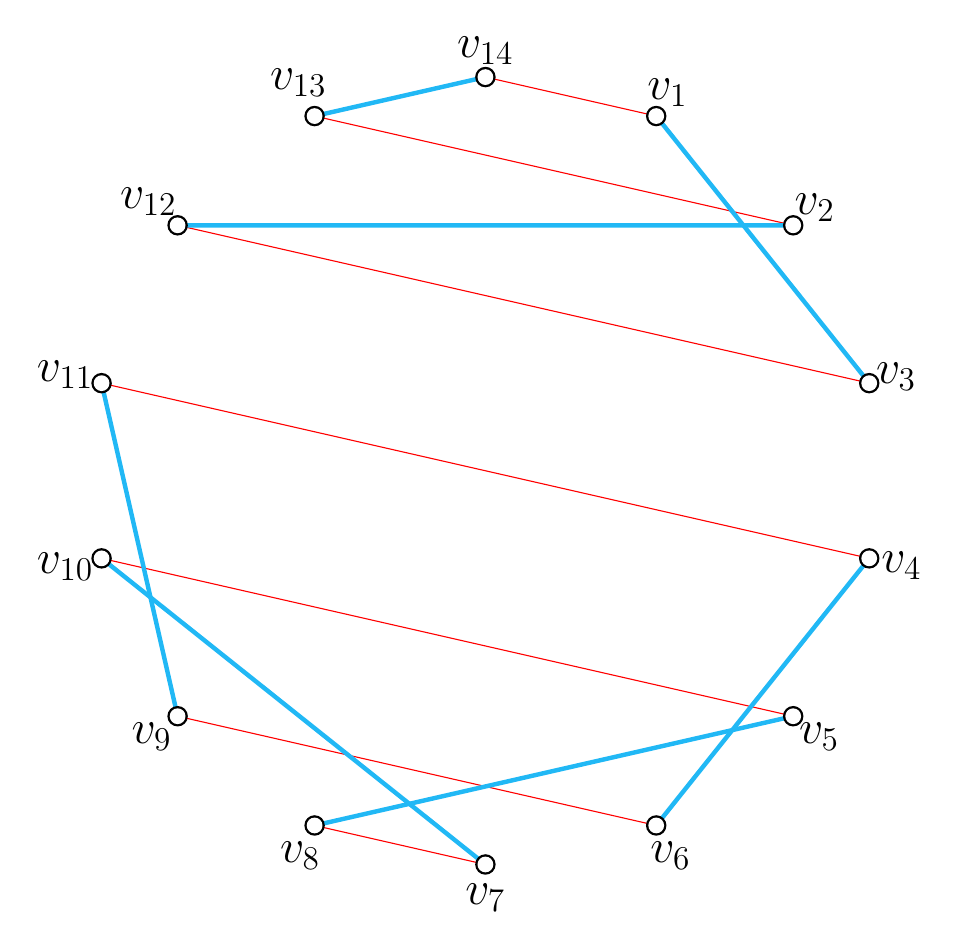
\begin{tikzpicture}
%Values of nodes:
% v1=1, v2=1, v3=2, v4=2, v5=2, v6=3, v7=3, v8=4, v9=4, v10=5, v11=5, v12=6, v13=7, v14=7 (v13/v14 universal vertices), \tau = 7.

\foreach \n/\value in {1/1, 2/1, 3/2, 4/2, 5/2, 6/3, 7/3, 8/4, 9/4, 10/5, 11/5, 12/6, 13/7, 14/7}
	\fill (90-\n*25.71428571:5cm) coordinate (v\n) circle [radius = 0.1];

\foreach \n/\value in {1/1, 14/14}
	\fill (90-\n*25.71428571:5cm) coordinate (v\n) circle [radius = 0.1]
		++(90-\n*25.71428571:9.5pt) node {\LARGE{$v_{\value}$}};

\foreach \n/\value in {2/2, 3/3}
	\fill (90-\n*25.71428571:5cm) coordinate (v\n) circle [radius = 0.1]
		++(90-\n*25.71428571:10pt) node {\LARGE{$v_{\value}$}};

\foreach \n/\value in {4/4, 5/5, 6/6, 7/7, 8/8, 9/9}
	\fill (90-\n*25.71428571:5cm) coordinate (v\n) circle [radius = 0.1]
		++(90-\n*25.71428571:12pt) node {\LARGE{$v_{\value}$}};

\foreach \n/\value in {10/10, 11/11, 12/12, 13/13}
	\fill (90-\n*25.71428571:5cm) coordinate (v\n) circle [radius = 0.1]
		++(90-\n*25.71428571:13.5pt) node {\LARGE{$v_{\value}$}};

\foreach \m/\n in {1/14, 2/13, 3/12, 4/11, 5/10, 6/9, 7/8}
	\draw [tRed] (v\n) -- (v\m);
\foreach \m/\n in {1/3, 2/12, 4/6, 5/8, 7/10, 9/11, 13/14}
	\draw [ultra thick, tBlue] (v\n) -- (v\m);
\foreach \n in {1,...,14}
	\fill (90-\n*25.71428571:5cm) coordinate (v\n) circle [radius = 0.13];
\foreach \n in {1,...,14}
	\fill [white] (90-\n*25.71428571:5cm) coordinate (v\n) circle [radius = 0.1];

\end{tikzpicture}
	
\end{document}